% Plastic lineages from the baseline treatment
\begin{figure*}[!ht]
  \centering
  \begin{minipage}[b]{\linewidth}
  \centering
  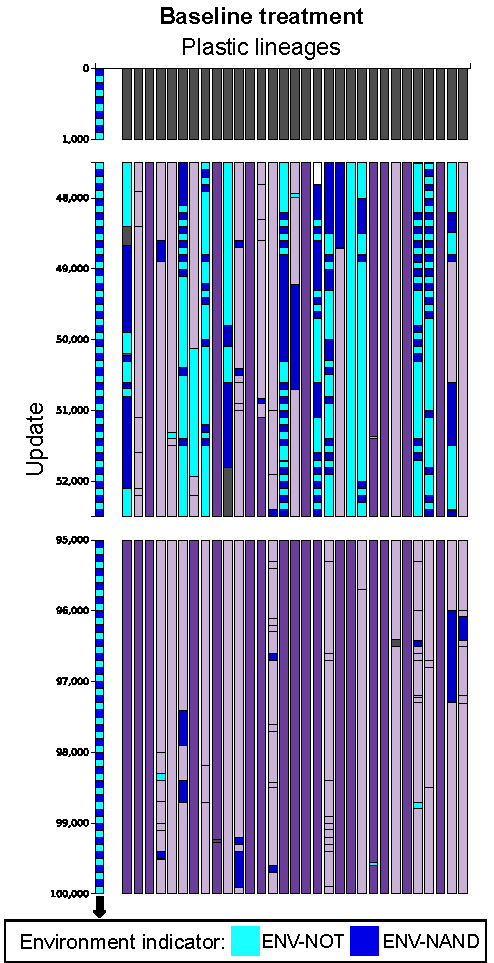
\includegraphics[height=0.5\textheight, keepaspectratio]{chapters/02-evolutionary-origins-of-plasticity/media/baseline-plastic-lineages.pdf}
  \caption{\small 
  Time-sliced lineage visualization of dominant, plastic genotypes from the baseline treatment. 
  Abbreviated color reference: 
  cyan represents unconditional NOT task performance, 
  dark blue represents unconditional NAND task performance, 
  light purple represents sub-optimal forms of plasticity, 
  and dark purple represents optimal plasticity.  
  Refer to Figure \ref{chapter:origins-of-plasticity:fig:task-profiles} for a full legend of phenotype colors.}
  \label{chapter:origins-of-plasticity:fig:baseline-lineages}
  \end{minipage}
\end{figure*}